\documentclass{beamer}


\usepackage[utf8]{inputenc}
\usepackage{lmodern} 
\usepackage[utf8]{inputenc}
\usepackage{lmodern} 
\usepackage{listings}
\usepackage{xcolor} 
\usepackage{graphicx}

\lstset{
	language=C,
	basicstyle=\ttfamily\small,
	keywordstyle=\color{blue},
	commentstyle=\color{green},
	stringstyle=\color{red},
	breaklines=true,
	breakatwhitespace=true,
	showstringspaces=false,
	frame=single,
	morekeywords={import, as, from, ctypes, numpy, matplotlib, pyplot, None},
	xleftmargin=0pt,
	framexleftmargin=0pt,
	aboveskip=0pt,
	belowskip=0pt
}




\definecolor{myblue}{RGB}{48, 63, 159}

\setbeamercolor{palette primary}{bg=myblue, fg=white}
\setbeamercolor{structure}{fg=myblue}
\setbeamercolor{frametitle}{bg=myblue, fg=white}
\setbeamercolor{title}{bg=myblue, fg=white}
\setbeamercolor{footlinecolor}{bg=myblue, fg=white}


\defbeamertemplate*{title page}{mytemplate}{
	\vfill
	\begin{center}

		\begin{beamercolorbox}[wd=0.8\paperwidth, center, rounded=true, shadow=true]{title}
			\usebeamerfont{title}\inserttitle\par
		\end{beamercolorbox}
		\vspace{2cm} 

		\usebeamerfont{author}\insertauthor
		\vspace{1cm} 
		\usebeamerfont{date}\insertdate
	\end{center}
	\vfill
}


\defbeamertemplate*{frametitle}{mytemplate}{
	\begin{beamercolorbox}[wd=\paperwidth, ht=2.5ex, dp=1.5ex, left]{frametitle}
		\hspace{1em}\usebeamerfont{frametitle}\insertframetitle
	\end{beamercolorbox}
}


\setbeamertemplate{footline}{
	\begin{beamercolorbox}[wd=\paperwidth, ht=2.25ex, dp=1ex]{footlinecolor}
		\hspace{1em}\usebeamerfont{author in footline}\insertshortauthor
		\hfill
		\usebeamerfont{title in footline}\insertshorttitle
		\hfill
		\usebeamerfont{date in footline}\insertdate \hspace{1em} \insertframenumber/\inserttotalframenumber \hspace{0.5em}
	\end{beamercolorbox}
}


\setbeamerfont{author in footline}{size=\tiny}
\setbeamerfont{title in footline}{size=\tiny}
\setbeamerfont{date in footline}{size=\tiny}



\title{1.10.16}
\author{Shriyansh Chawda-EE25BTECH11052}
\date{August 23, 2025}



\begin{document}
	

		\setbeamertemplate{footline}{} 
		\frame{\titlepage}
	
	
	

	\begin{frame}{Question} 
			The unit vector in the direction of x is
	\end{frame}
	
	

	\begin{frame}{Solution}

The unit vector in the direction of x is
\begin{equation}
	\frac{\mathbf{x}}{\|\mathbf{x}\|} \tag{1.1.8.1}
\end{equation}

Given the vector $\mathbf{a} = 2\hat{i} + 3 \hat{j} + \hat{k}$.
The magnitude of vector $\mathbf{a}$:$$ \|\mathbf{a}\| = \sqrt{2^2 + 3^2 + 1^2} = \sqrt{4+9+1} = \sqrt{14} \quad (1)$$Then, the unit vector in the direction of $\mathbf{a}$ is found by dividing the vector by its magnitude:$$\implies \frac{\mathbf{a}}{\|\mathbf{a}\|} = \frac{1}{\sqrt{14}} \begin{pmatrix} 
	2 \\ 
	3 \\ 
	1 
\end{pmatrix} 
$$
\end{frame}
\begin{frame}
\begin{figure}[h!]
	\centering
	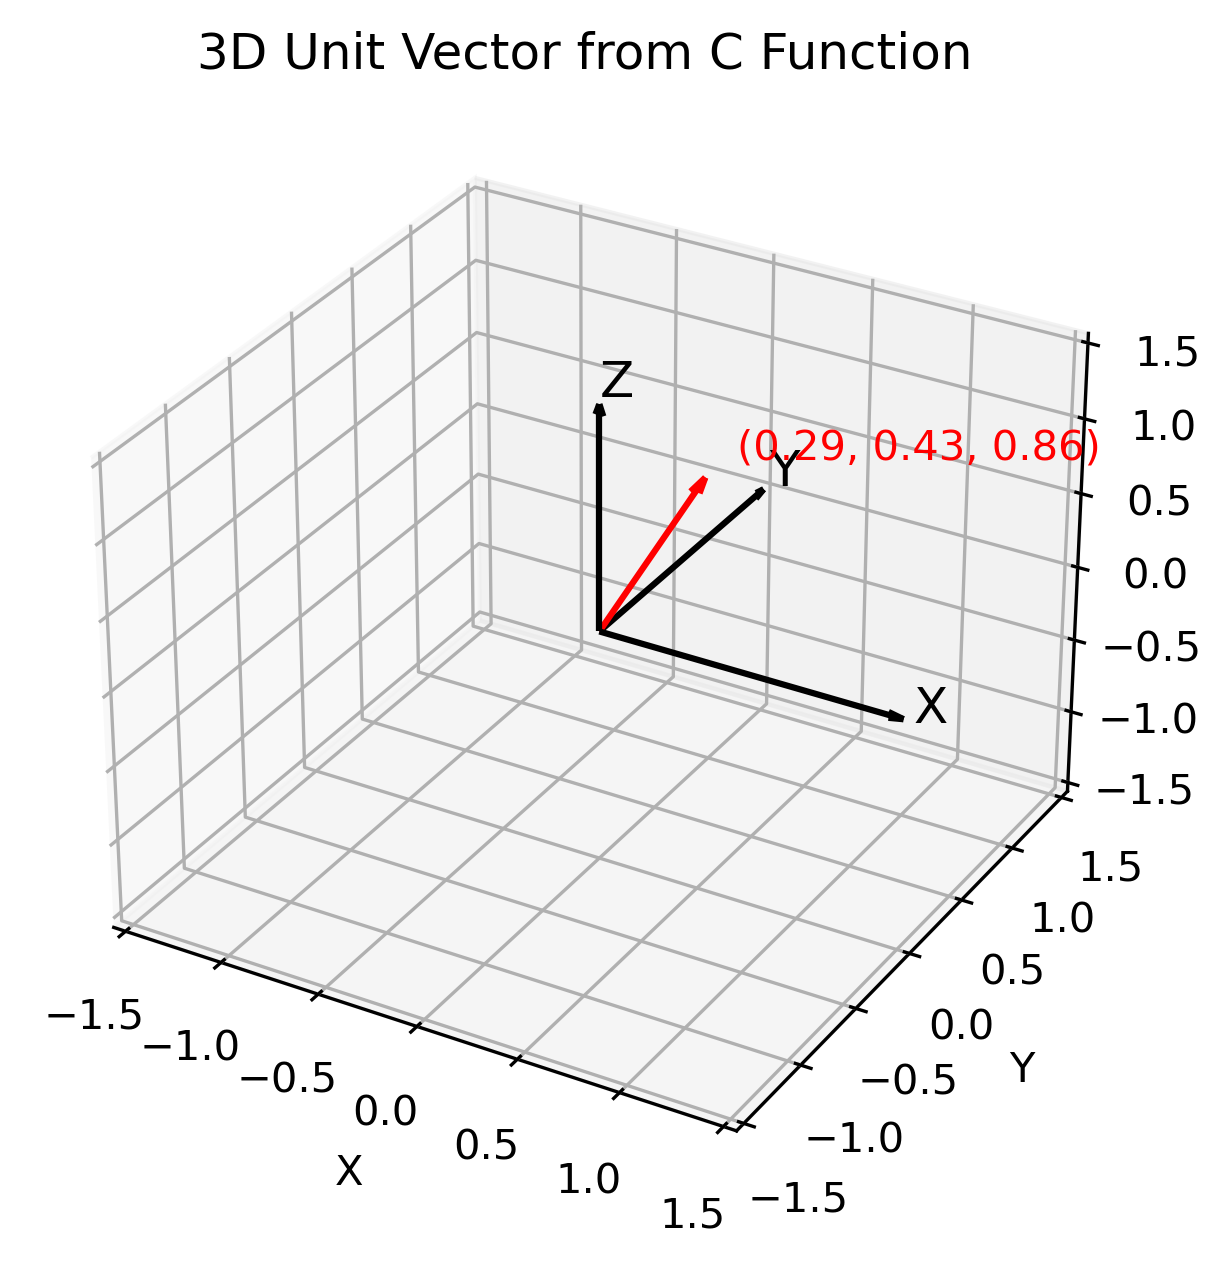
\includegraphics[width=0.5\linewidth]{figs/unit_vector3d}
	\label{fig:unitvector3d}
\end{figure}


\end{frame}



\end{document}